\textit{In this document, "TensorShape", "Tensor", and "TensorArray" that begin with a capital letter particularly refer to a type, while "tensor shape", "tensor" and "tensor array" refer to the general concpet.}

\section{Basic concepts}

\subsection{TensorShape}

TensorShape $S=<S_1,S_2,...,S_n>$ is a tuple of $n$ non-negative integers that specify the size of each dimension of a tensor.

\begin{itemize}
  \item TensorShape is a collection of non-negative integers which are \textbf{ordered} and \textbf{immutable}.
  \item TensorShape is iterative. Its elements can be traversed through sequentially.
  \item TensorShape is written as two parentheses containing integers in it.
\end{itemize}

\begin{lstlisting}[language=Python]
(3,5,3)
() # empty tuple ?
\end{lstlisting}

\textcolor{red}{[TBD]: encode uncontrolled dimension and inform its range.}

\subsection{Tensor}

A dense Tensor is a \textbf{\textit{fixed-size multi-dimensional}} container of primary arithmetic type. A tensor x:Tensor is characterized by meta data:
\begin{enumerate}
  \item elemental type T, including basic arithmetic type: real, bool, integer.
  \item shape $S(\text{x})$: shape defines multi-dimensional indices, each index access decides the physical location of an item stored in the tensor.
  \item \textcolor{red}{layout: the order that each dimension is stored}.
\end{enumerate}

The $n$ dimensions of a tensor canbe stored in any order. A $n$-dimensional tensor is a \textbf{\textit{$n$-way collection of numbers with primary arithmetic type}}. Data stored in a tensor can be accessed from $n$ directions, but a high-dimensional tensor can only be accessed efficiently in one direction. Figure \ref{fig1} shows the idea.

\begin{figure}[htbp]
\centering
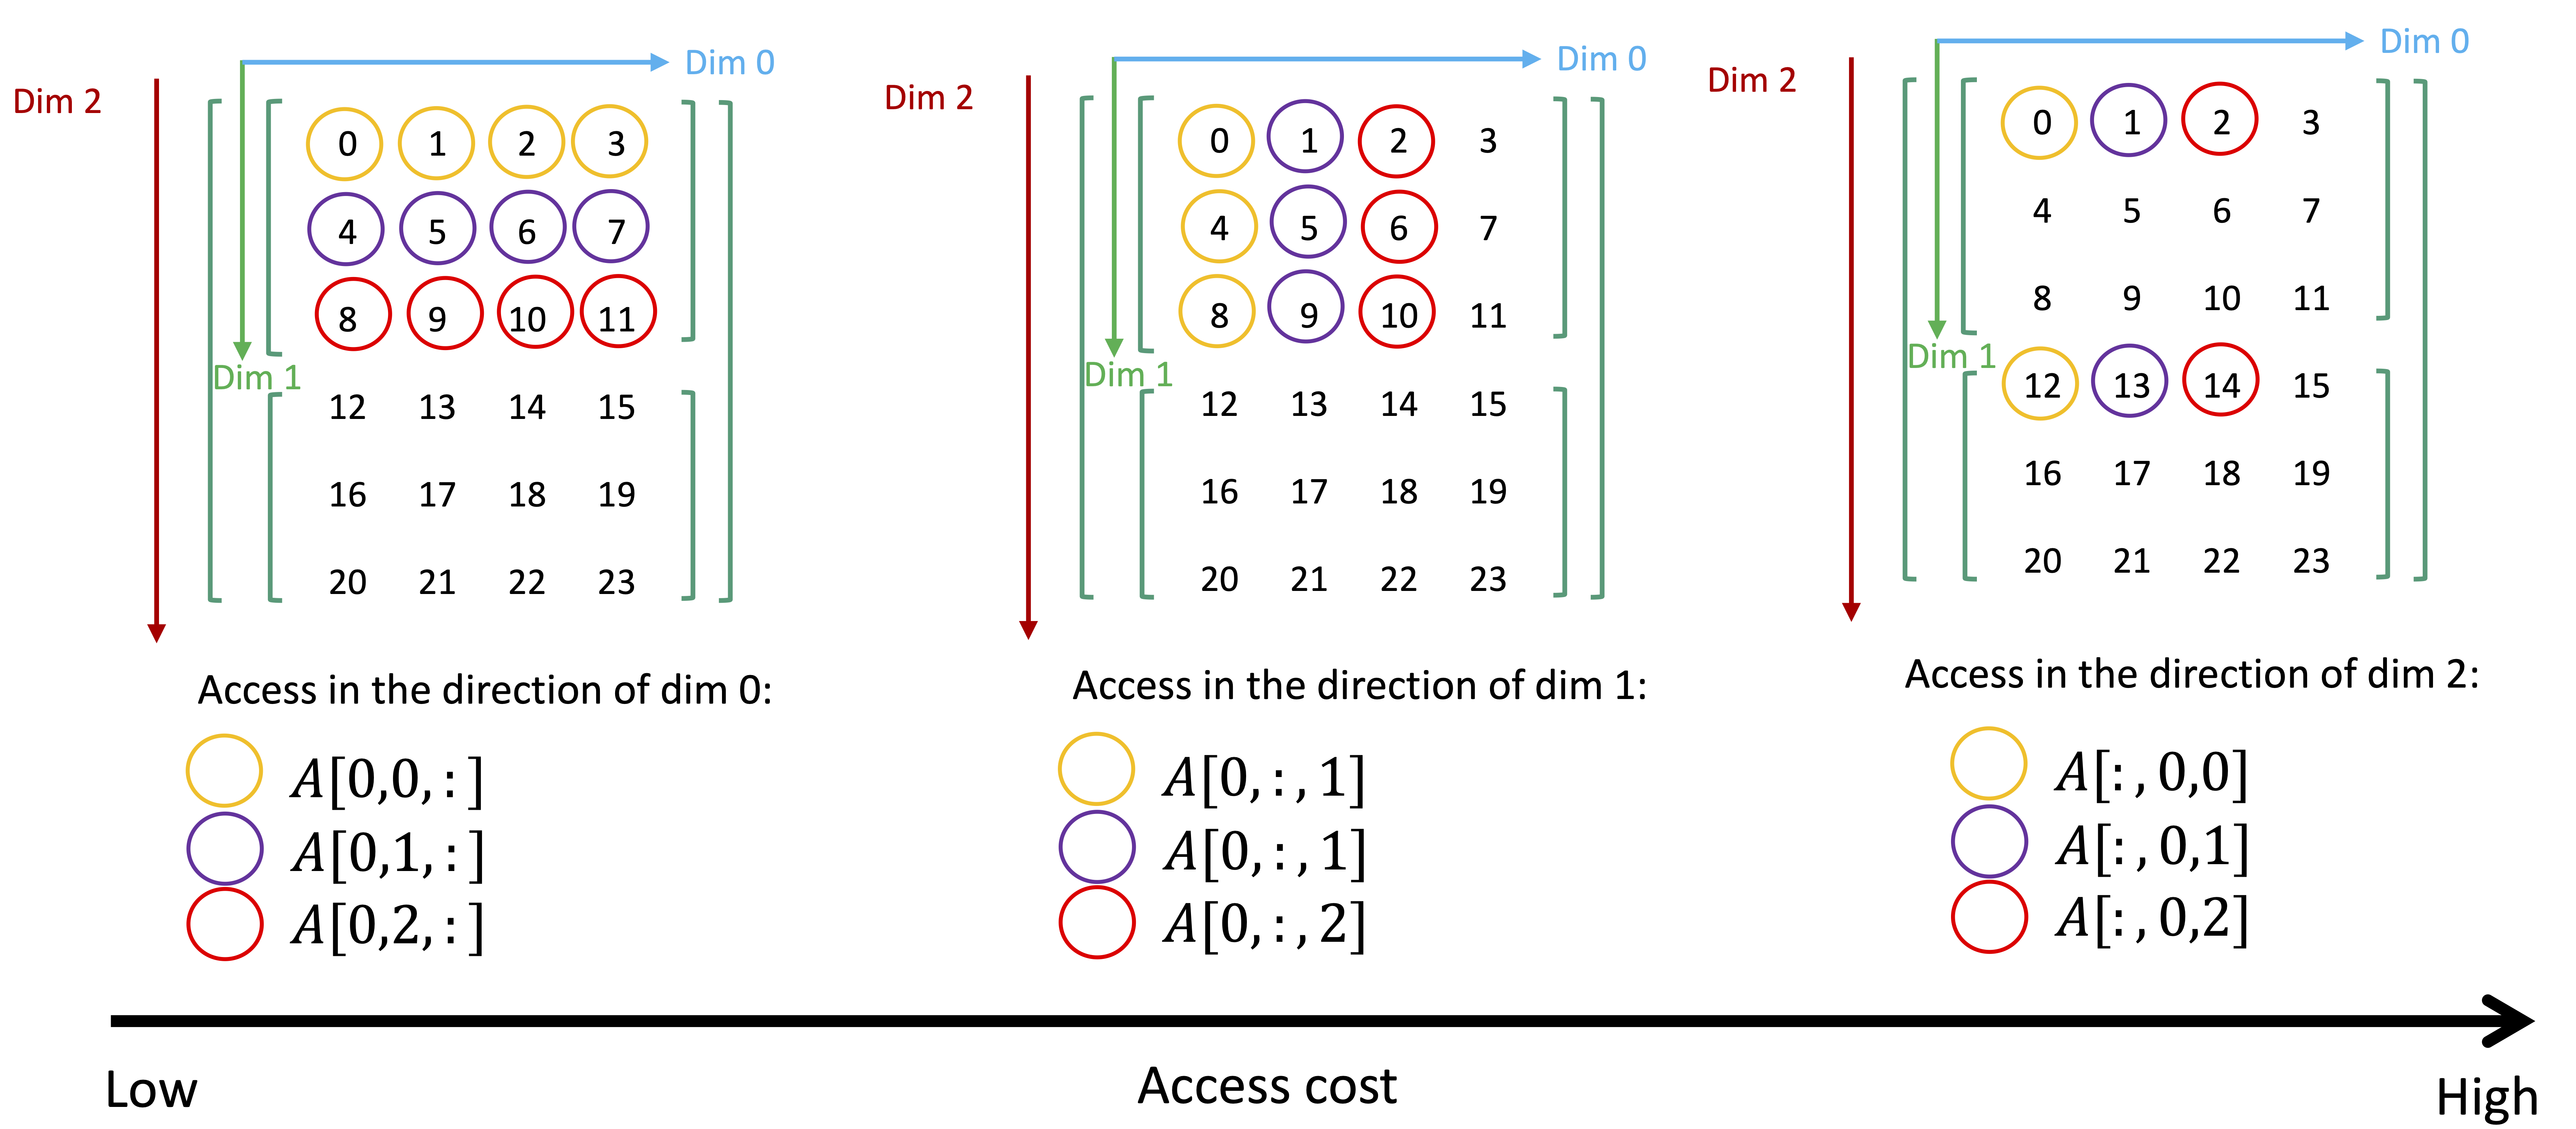
\includegraphics[width=1.\textwidth]{images/tensor.png}
\caption{Access a 3-d tensor.}
\label{fig1}
\end{figure}

\subsection{TensorArray}

A TensorArray is a \textbf{\textit{variable-size one-dimensional list-like}} container of fixed-size tensors or tensor arrays. Items in a TensorArray can either be Tensors or TensorArrays. A $n$-depth nested TensorArray is a \textbf{\textit{$n$-way collection of fixed-size Tensors}}. TensorArray can be analogous to std::vector<T> in C++, where T = Tensor or TensorArray.

For a tensor array x:TensorArray[T], T is either:

\begin{enumerate}
  \item T = Tensor called a primary TensorArray. For a primary TensorArray, all tensors stored in x \textbf{\textit{should be homogenous}}. That is, every tensor takes up the same size block of memory, and all blocks are interpreted in exactly the same way.
  \item T = TensorArray indicates a nested tensor array. For a nested tensor array, tensors stored in all depths should have a same primary arithmetic type and a same shape. \textcolor{red}{[TBD]: how flexible a TensorArray should be?}
\end{enumerate}

A tensor array x:TensorArray[T] is characterized by meta info:
\begin{enumerate}
  \item elemental type T that is either Tensor or TensorArray.
  \item length $L(\text{x})$: length defines one-dimensional indices, and maximum length is declared.
\end{enumerate}

Nested tensor array provides a constraint way to encode sparsity on the basis of high-level abstraction tensor. The constrain requires indices in a single tensor array are continous. Future work that extends the internal storage format of TensorArray and optimizes accessing methods for such a format could make TensorArray supports general sparsity.

\subsubsection{Motivations for TensorArray}

Main purposes of introducing the TensorArray abstraction include:
\begin{enumerate}
  \item Provides a flexible data structure to boundle data that are not as regular as tensors.

  \begin{itemize}
    \item A nested tensor array forms a rectangular polyhedron in high-dimensional space, providing a way for users to encode structural data.
  \end{itemize}

  \item Raise the abstraction level of data unit manipulated in the computation.
  \begin{itemize}
    \item Many optimized linear algebra routines are performed on blocks of memory and algorithm developers do not care more details about scalar-level computations. Based on these observations, nested tensor array provides a logic bundle of a set of large memory blocks. The deeper tensor arrays are nested, the larger memory is involved, and more opportunities to exploit parallelism and to reduce the overhead of item access are exposed.
    \item Iterating and accessing tensor arrays derive its performance from the compile-time analysis.
    \item TensorArray raises the abstraction level of Tensor. Interfaces to access items and iterate through Tensor and TensorArray share many similarities. They could be interconvertible through internal reasoning. High-level abstraction helps trade-off analysis complexity with global optimality.
  \end{itemize}

  \item Enable precise memory-based dependence analysis to improve program parallelism.

  \begin{itemize}
    \item Parallel patterns become implicit for algorithms that iterate over \textit{\textbf{nested}} tensor arrays using nested looping constructs. TensorArray abstracts away low-level details of underlying memory, and makes dependence analysis simplified with the help of high-level abstractions.
  \end{itemize}

  \item Separate the effects and interfaces of operations applied to fixed-size and variable-size memory blocks which also cause different storage formats and memory management internally.

  \begin{itemize}
    \item Undecidable memory size at compile-time leads to dynamics. TensorArray operations will delegate to different implementations according to whether compile-time analysis can reason about strong static conditions of a tensor array.
  \end{itemize}

\end{enumerate}

\subsubsection{Shape of a nested TensorArray}

Tensors in tensor arrays and nested tensor arrays are stored in a continous memory. Shape of nested tensor array, a meta data, is in the form of a tree. Figure \ref{nested_ta} shows the intuitioin.

\begin{figure}[htbp]
\centering
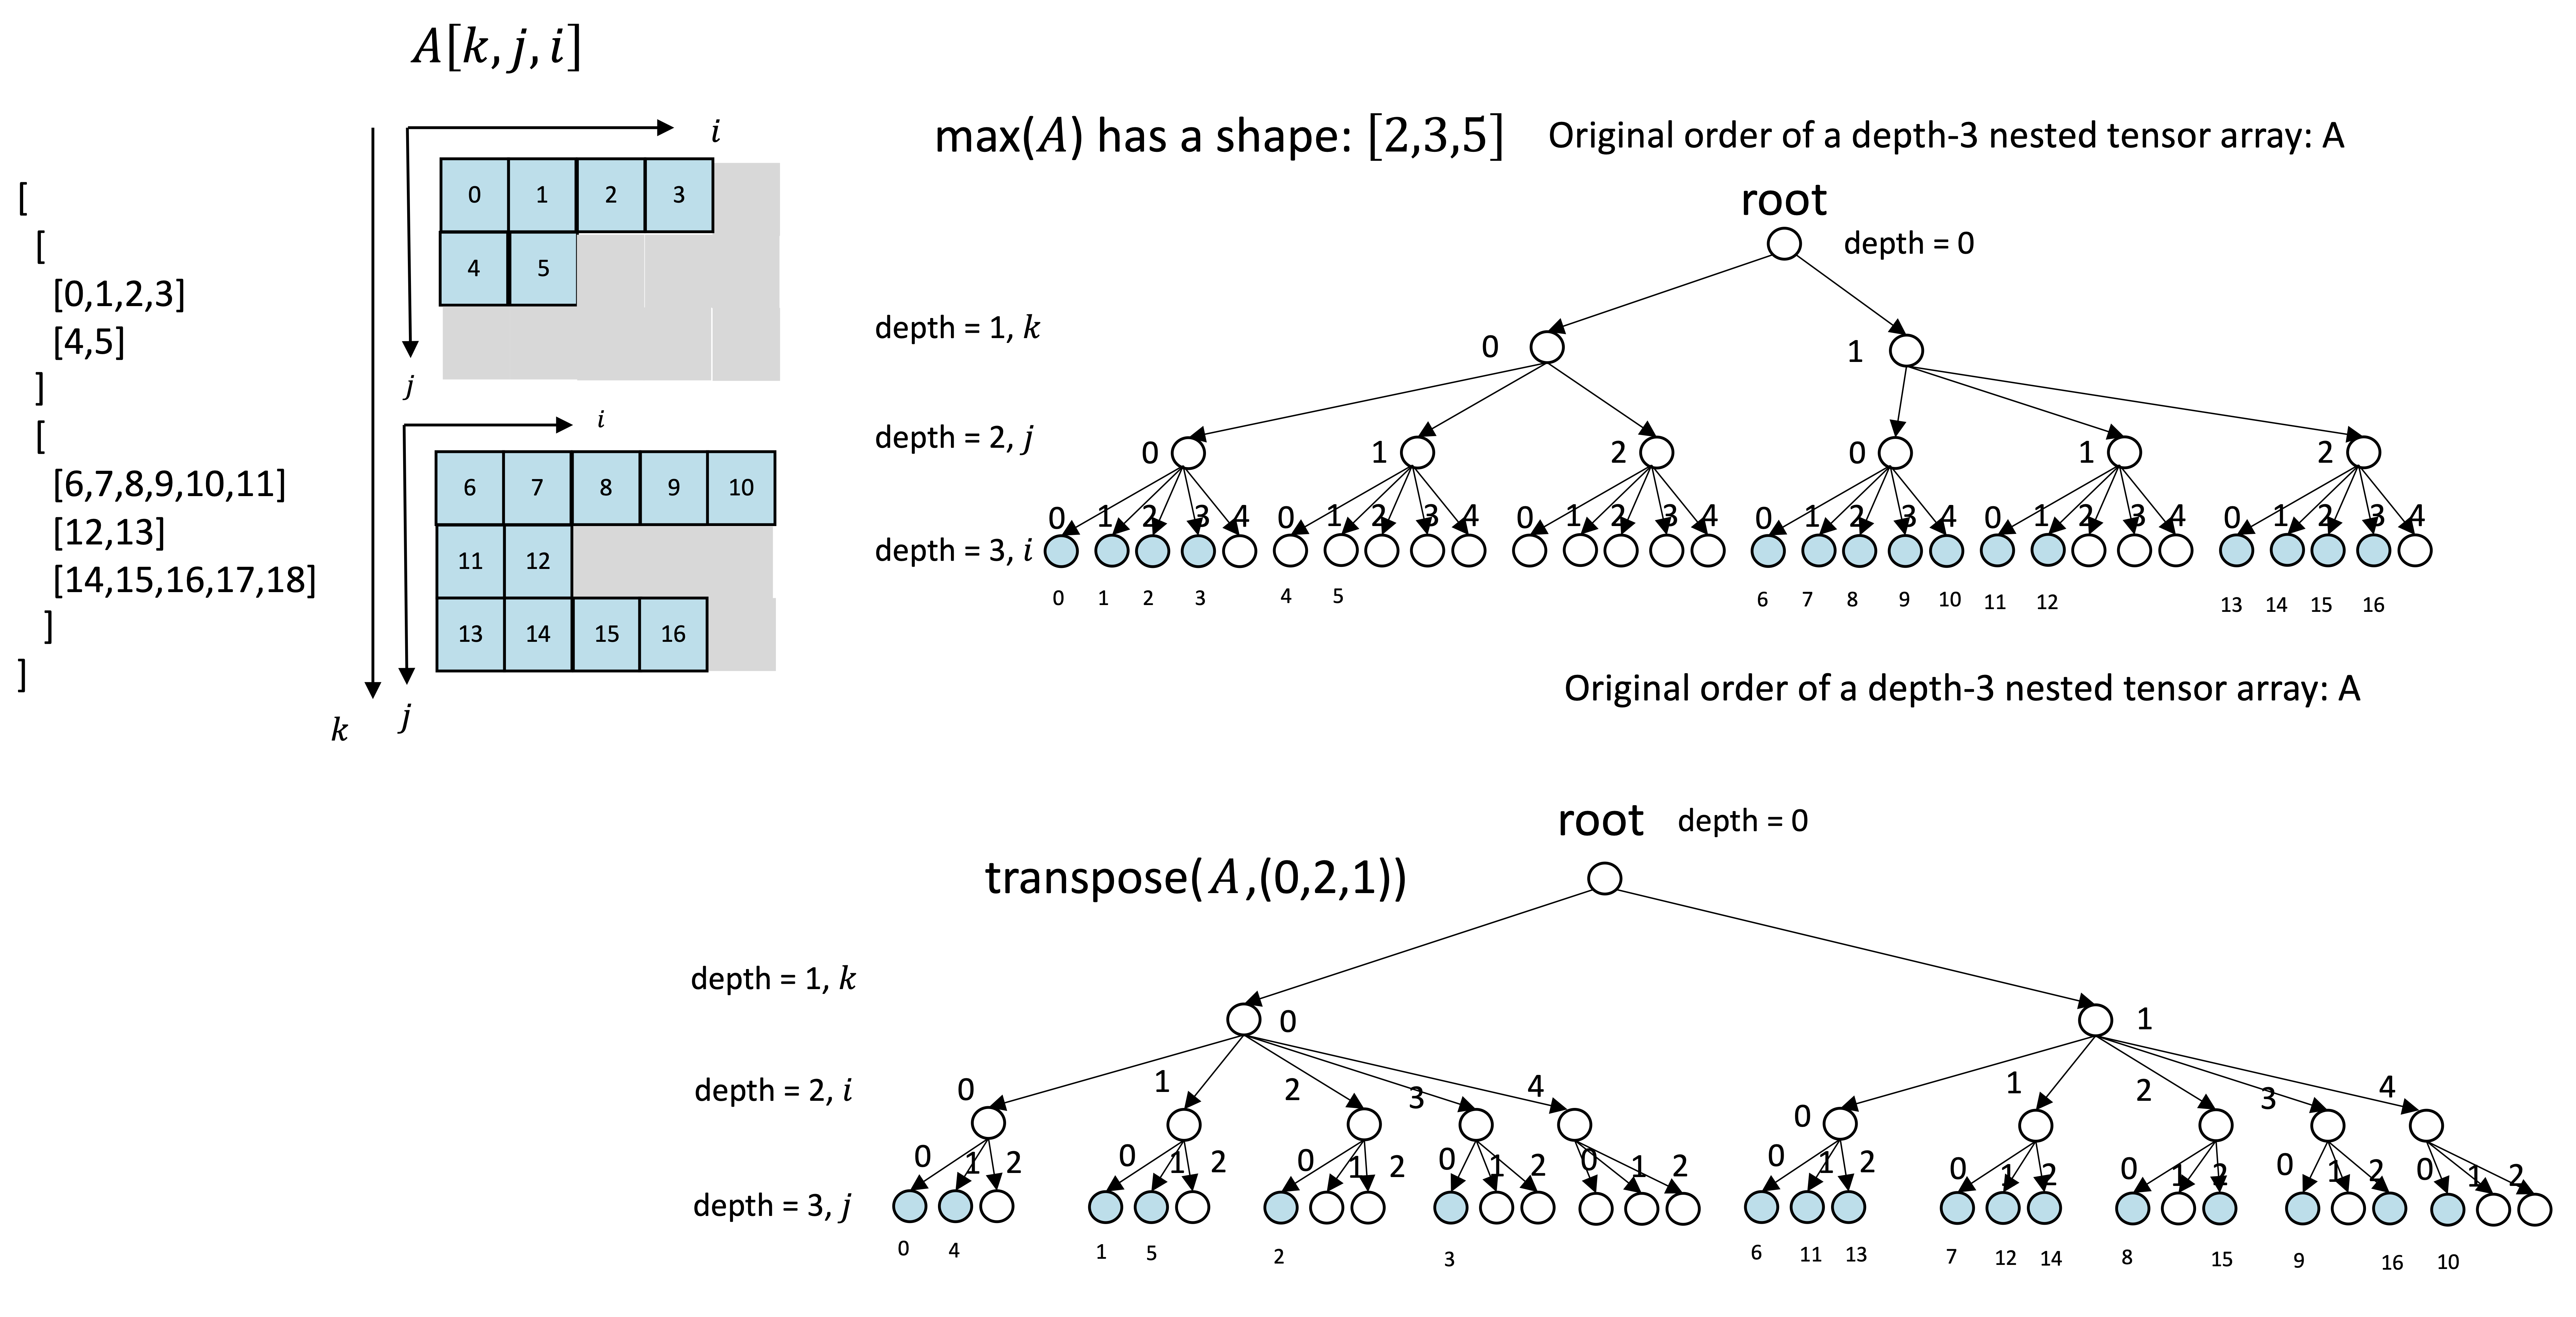
\includegraphics[width=1.\textwidth]{images/nested_tensorarray.png}
\caption{A conceptual diagram of the nested tensor array.}
\label{nested_ta}
\end{figure}
